\documentclass{article}
\author{Victor Mittermair, 11809916}
\usepackage{hyperref}
\usepackage{fancyhdr}
\usepackage{tikz} 
\usepackage{amsthm}
\usepackage{verbatim}
\usepackage{subfigure}
\usepackage{amssymb}
\usepackage{mathtools}
\usepackage{amsmath}
\usepackage{soul}
\usepackage{algorithm}
\usepackage{algpseudocode}
\usepackage{algorithmicx}
\usepackage{enumerate}

\newtheorem*{theorem}{Theorem}
\newtheorem*{lemma}{Lemma}
\theoremstyle{definition}
\newtheorem*{definition}{Definition}
\theoremstyle{remark}
\newtheorem*{remark}{Remark}
\newtheorem*{note}{Note}
\newtheorem*{statement}{Statement}
\newtheorem*{example}{Example}

%\lhead{\includegraphics[width=0.2\textwidth]{nyush-logo.pdf}}
\fancypagestyle{firstpage}{%
  \lhead{TU Vienna}
  \rhead{
  Discrete Math for Informatics WS 2022}
}

%%%% PROJECT TITLE
\title{Discrete Math for Informatics\\
        \Large \emph{5th Lecture}}


\date{\today} %NO DATE



\begin{document}
\maketitle
\thispagestyle{firstpage}


\begin{comment}
\section*{Graph}
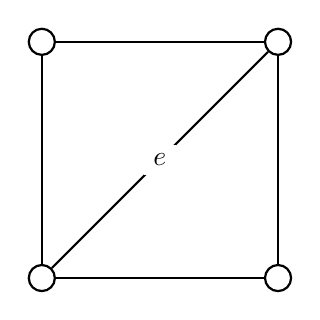
\begin{tikzpicture}[node distance={30mm}, thick, main/.style = {draw, circle}]
    \centering
    \node[main] (1)              {}; 
    \node[main] (2) [right of=1] {};
    \node[main] (3) [below of=1] {}; 
    \node[main] (4) [right of=3] {};
    \draw (1) -- (2) ; 
    \draw (1) -- (3); 
    \draw (2) -- (4); 
    \draw (3) -- (4);
    \draw (3) -- (2) node [midway, fill=white] {$e$}; 
\end{tikzpicture}
\end{comment}
\begin{definition}
  $S \subseteq V, s \in S , t \notin S$ then $(S, V \backslash S)$ is a \textbf{cut}, any edge from $S$ to $V\backslash S$ is called \textbf{crossing} the cut.
  $$c(S, V\backslash S) = \sum_{(u,v) \ in E ; u\in S, v\notin S} w(u,v)$$ is the \textbf{capactiy} of a cut.\\
  A cut is \textbf{minimal} if its capactiy is minimal along all cuts.\\
  A flow is \textbf{maximal} if its value is maximal among all flows.
\end{definition}
\begin{lemma}
  $val(\phi) \leq c(S,V\backslash S)$ for any flow $\phi$ and all cuts $c(S, V\backslash S)$ 
\end{lemma}
\begin{proof}
  \begin{equation*}
    val(\phi) = \sum_{(u,v) \in E; u\in S, v\in V \backslash S}\phi(u,v) - \sum_{(u,v) \in E; v\in S, u\in V \backslash S}\phi(u,v) \leq c(S, V \backslash S)
  \end{equation*}
  graph 1
  because $$ \begin{aligned} \text{inner sum = 0 if s = v} val(\phi) &= \sum_{v\in S} (\sum_{(v,u) \in E}\phi(v,u) - \sum_{(u,v) \in E} \phi(u,v)) \\
    &= \sum_{(v,u) \in E; v\in S, u\in V \backslash S}\phi(v,u) - \sum_{(u,v) \in E; v\in S,u\in V \backslash S}\phi(u,v)
  \end{aligned}$$
  
\end{proof}
\begin{definition}
  An \textbf{augmenting path} $P$ for $\phi$ is (unoriented) path from $s$ to $t$ with \\
  $\phi(e) < w(e) \forall e \in P$ traversed in the forward direction.\\
  $\phi(e) > 0 \forall e \in P$ traversed in the backward direction. 
\end{definition}
\begin{theorem}
  Let $\phi$ be any flow, then\\
   $val(\phi)$ is maximal $\Longleftrightarrow \nexists $ augmenting path for $\phi$\\
   $val(\phi)$ is maximal $\Longleftrightarrow val(\phi) = c(S, V\backslash S)$ for some $S$
\end{theorem}
\begin{proof}
  $val(\phi)$ is max $\Rightarrow \nexists $ augmenting path for $\phi$\\
  suppose $P$ is an augmenting path,\\ let $\delta_1 := min_{e\in P;forward}(w(e)-\phi(e)), \delta_2:= min_{e\in P;backward}(\phi(e)) \delta:= min(\delta_1, \delta_2)$
  function 1
  $\widetilde{\phi}$ is a flow: check $F2$ for a vertex $v$ on the path.
  $$\sum_{(v,u) \in E} \widetilde{\phi}(e) = \sum_{(v,u) \in E} \phi(e) + $$ function 2\\
  $\nexists$ augmenting path $\Rightarrow$ property 2 of theorem.\\
  let $S=\{v \in V | \exists \text{"augmenting path" from s to v} \}$\\
  $(S, V\backslash S)$ is a cut (because $s\in S$).\\
  for forward crossing edges we have $\phi(e)=w(e)$ in this cut\\
  for backward crossing edges we have $\phi(e)=0$\\
  use lemma $val(\phi)= \sum_{e forward}\phi(e)-\sum_{e backward}\phi(e)=c(S, V\backslash S)-0$\\
  graph 2
  graph 3\\
  property 2 $\Rightarrow$ $val(\phi)$ is maximal.\\
  Lemma: $val(\phi) \leq c(S, V\backslash T)$, so $val(\phi)$ is maximal.
\end{proof}
\begin{theorem}
  A maximal flow exists.
\end{theorem}
\begin{proof}
  if $w:E\rightarrow \mathbb{N}$ an augmenting path increases $val(\phi)$ by at least one.\\
  if $w:E\rightarrow \mathbb{Q}$ multiply all weights by the lcm of the denominators.\\
  if $w:E\rightarrow \mathbb{R}$ any continous real function on a compact set has a maximum.
\end{proof}
\begin{remark}
  val of max flow = capacity of a min cut. (Max-Flow-Min-Cut theorem)
\end{remark}
\begin{algorithm}
  Ford-Fulkerson algorithm: 
  \begin{algorithmic}
  \State $\phi_1(e) \gets 0$ for all e
  \While{$\exists$ augmenting path $P$ for $\phi_i$}
     \State function 3
  \EndWhile
  \end{algorithmic}
\end{algorithm}
\subsection*{Hall's marriage theorem}
$X,Y$ finite disjoint sets $|X|=|Y|$, $D\subseteq X \text{x} Y$
\begin{definition}
  a \textbf{perfect matching} $M\subseteq D$ s.t. $\forall x\in X \exists ! y\in Y: (x,y) \in M$
\end{definition}
\begin{theorem}
  $D$ admits a perfect matching $\Longleftrightarrow$ $\forall X^\prime \subset X: |N^+(X^\prime)| \geq |X^\prime|$
\end{theorem}
\begin{proof}
  $\Rightarrow$ use the perfect matching, every $x$ is matched to a different $y$\\
  $\Leftarrow$, graph 4, the value of the max flow is the size of the largest matching.\\
  let $(\{s\}\cup \widetilde{X} \cup \widetilde{Y}, X \backslash \widetilde{X} \cup Y \backslash \widetilde{Y} \cup \{t\})$ be a minimal cut.\\
  $\widetilde{Y} \supseteq N^+(\widetilde{X})$ because $w(x,y) = \infty$\\
  $c(S, V\backslash S) = |X\backslash \widetilde{X}| + |\widetilde{Y}|$\\
  $c(S, V\backslash S) \geq |X|$ because $|\widetilde{Y}| \geq |N^+(\widetilde{X})| \geq |\widetilde{X}|$ and $|X\backslash \widetilde{X}|+|\widetilde{Y}| \geq |X\backslash \widetilde{X}|+ |\widetilde{X}| = |X|$
\end{proof}
\end{document}